\documentclass{article}
\usepackage{graphicx} %package to manage images
\graphicspath{ {./figures/} }
\usepackage{hyperref}
\usepackage{caption}
\usepackage[font=scriptsize]{subcaption}
\captionsetup[figure]{labelsep=none}
\captionsetup[table]{labelsep=none}
\usepackage{bbm}
\usepackage{amsmath}
\usepackage{import}
\usepackage{array}
\usepackage{booktabs}
\usepackage{afterpage}
\usepackage{floatrow}
\usepackage{pdflscape}
\usepackage{soul}
\usepackage{float}
\usepackage{adjustbox}
\usepackage{longtable}


\title{trends in health in pregnancy (overleaf)}

\date{April 2025}

\begin{document}

\maketitle



TODO
- add short note after each figure/table and about how it was generated
\begin{figure}[H]
    \centering
    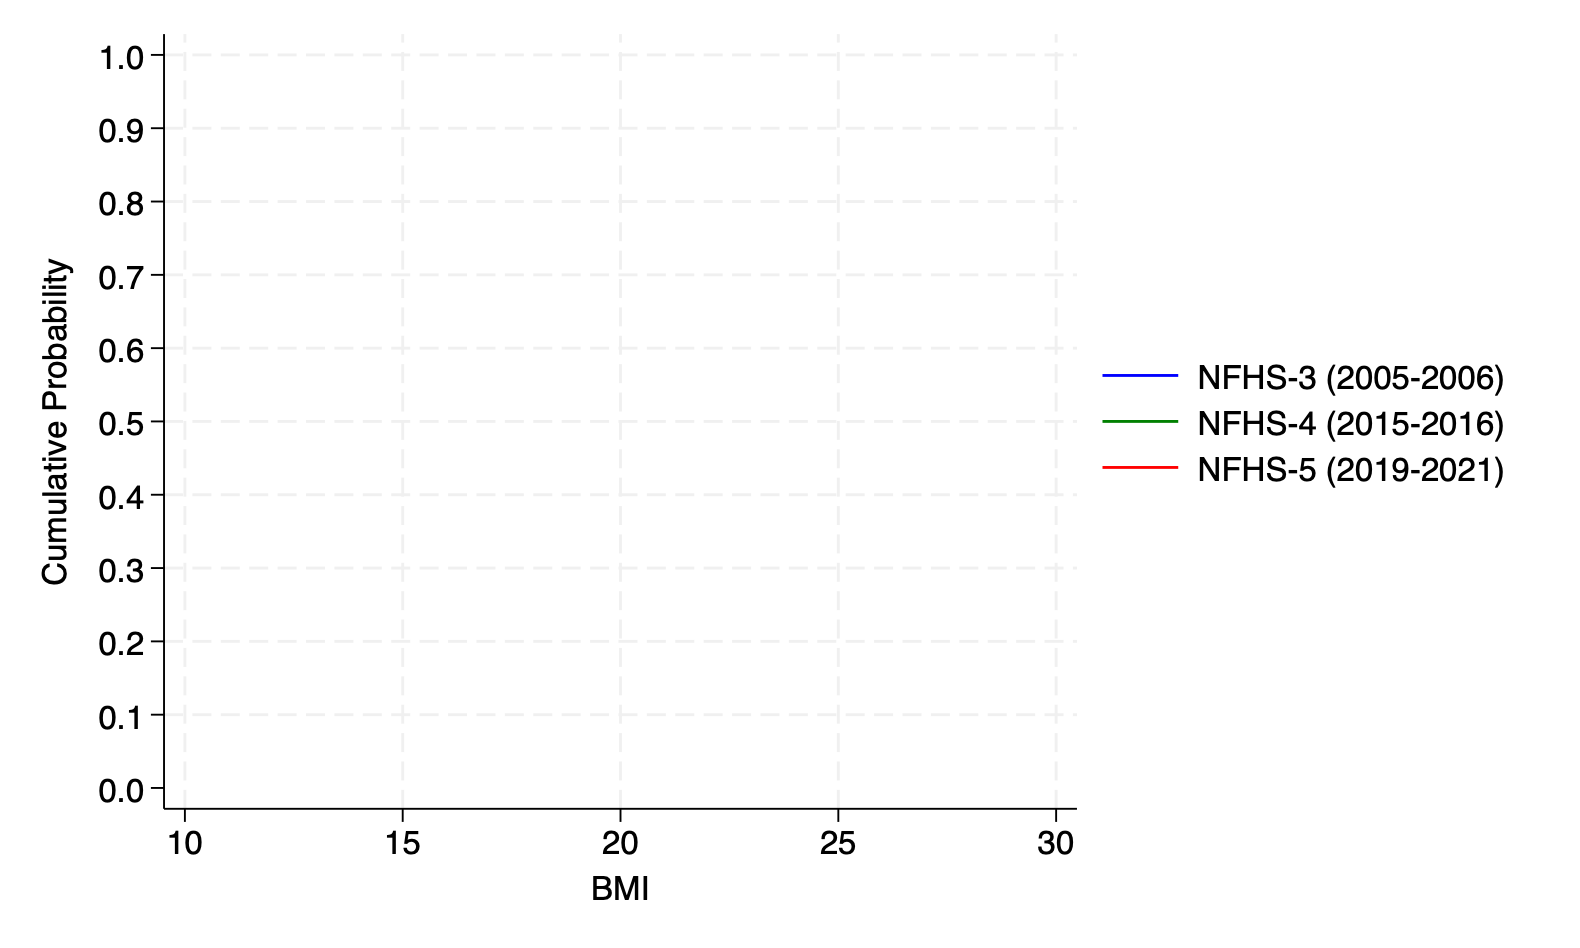
\includegraphics[width=\textwidth]{figures/cdf prepregnancy bmi.png}
    \caption{: CDFs of Estimated Pre-Pregnancy BMI in NFHS 3, 4, \& 5}
    
\end{figure}



\begin{figure}[H]
    \centering
    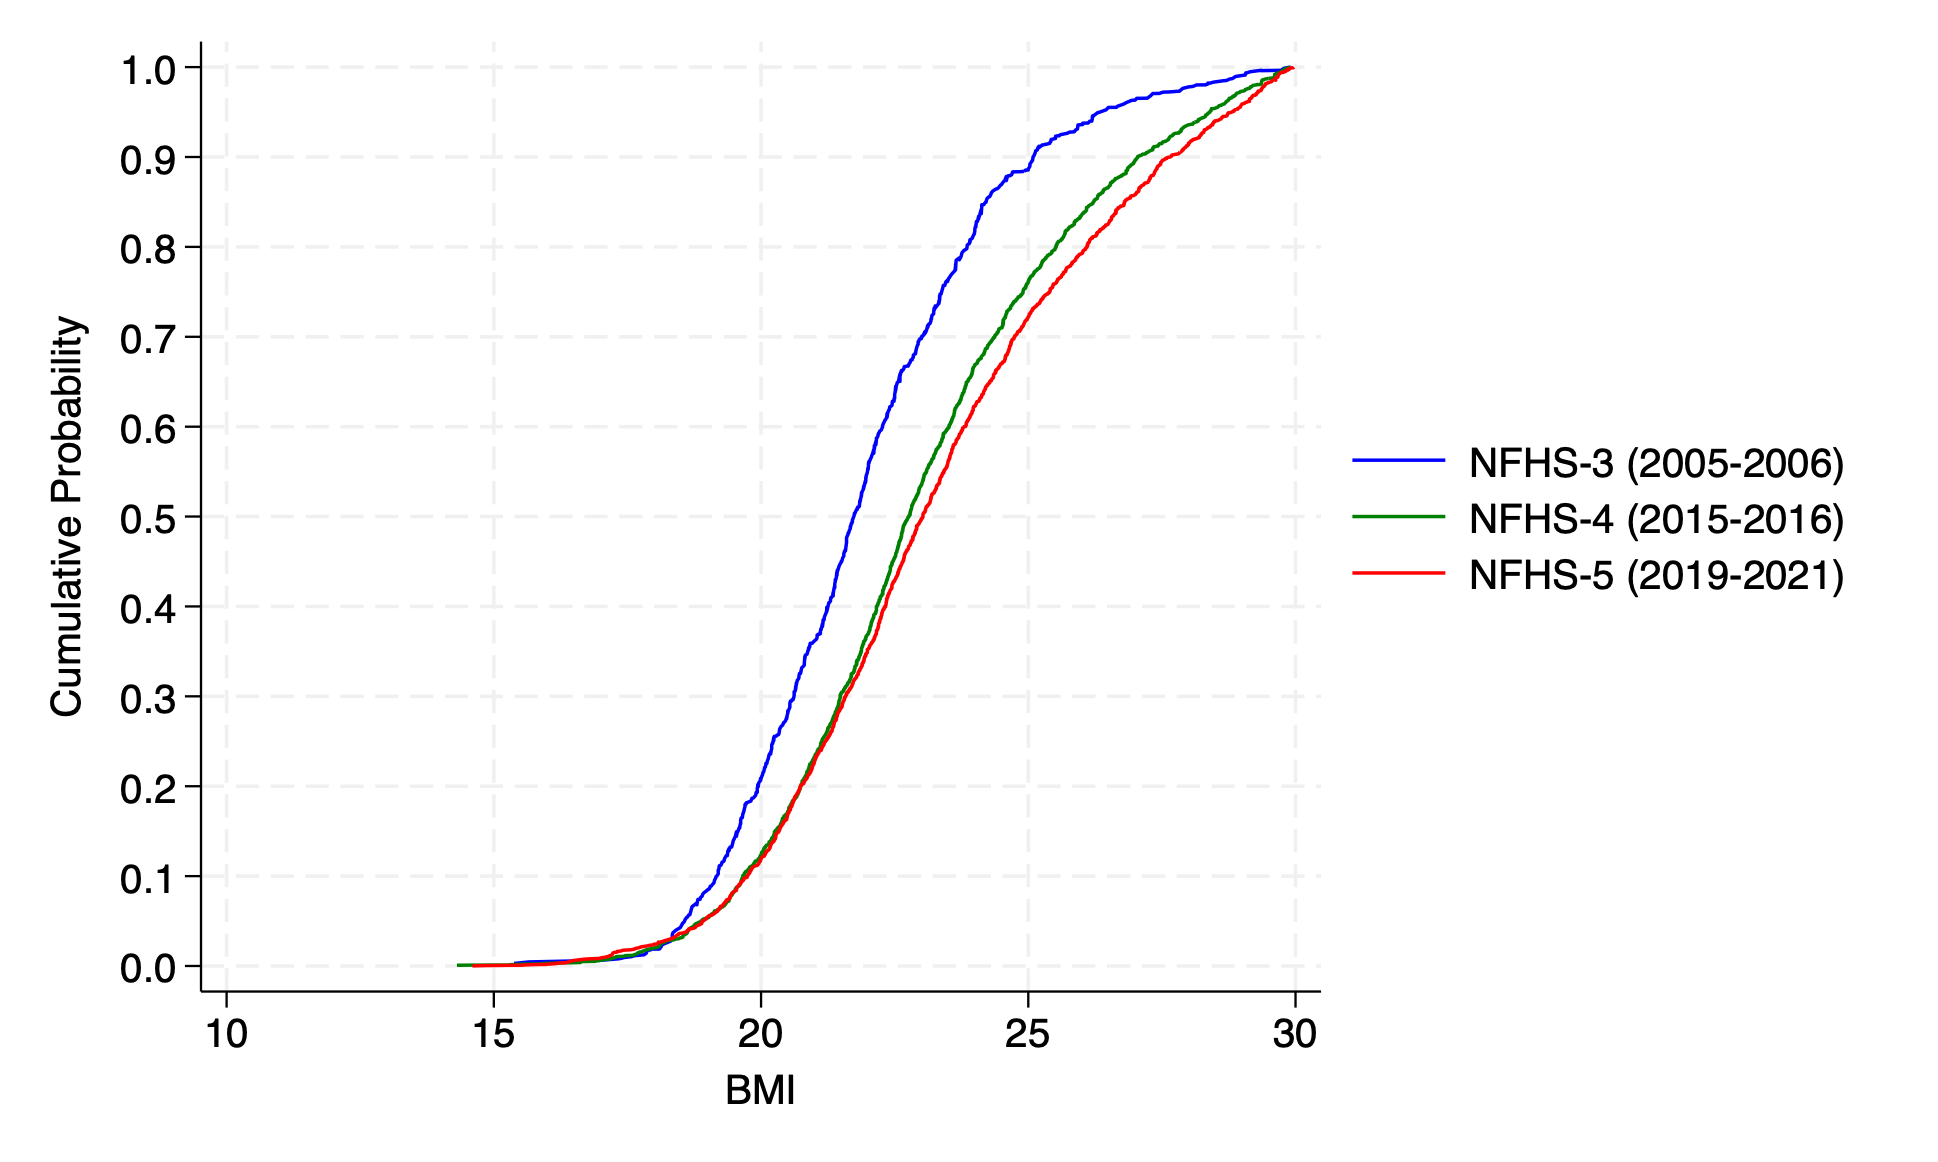
\includegraphics[width=\textwidth]{figures/cdf nine months bmi.png}
    \caption{: CDFs of Observed BMI at 9+ months pregnant in NFHS 3, 4, \& 5}
    
\end{figure}


\begin{figure}[H]
    \centering
    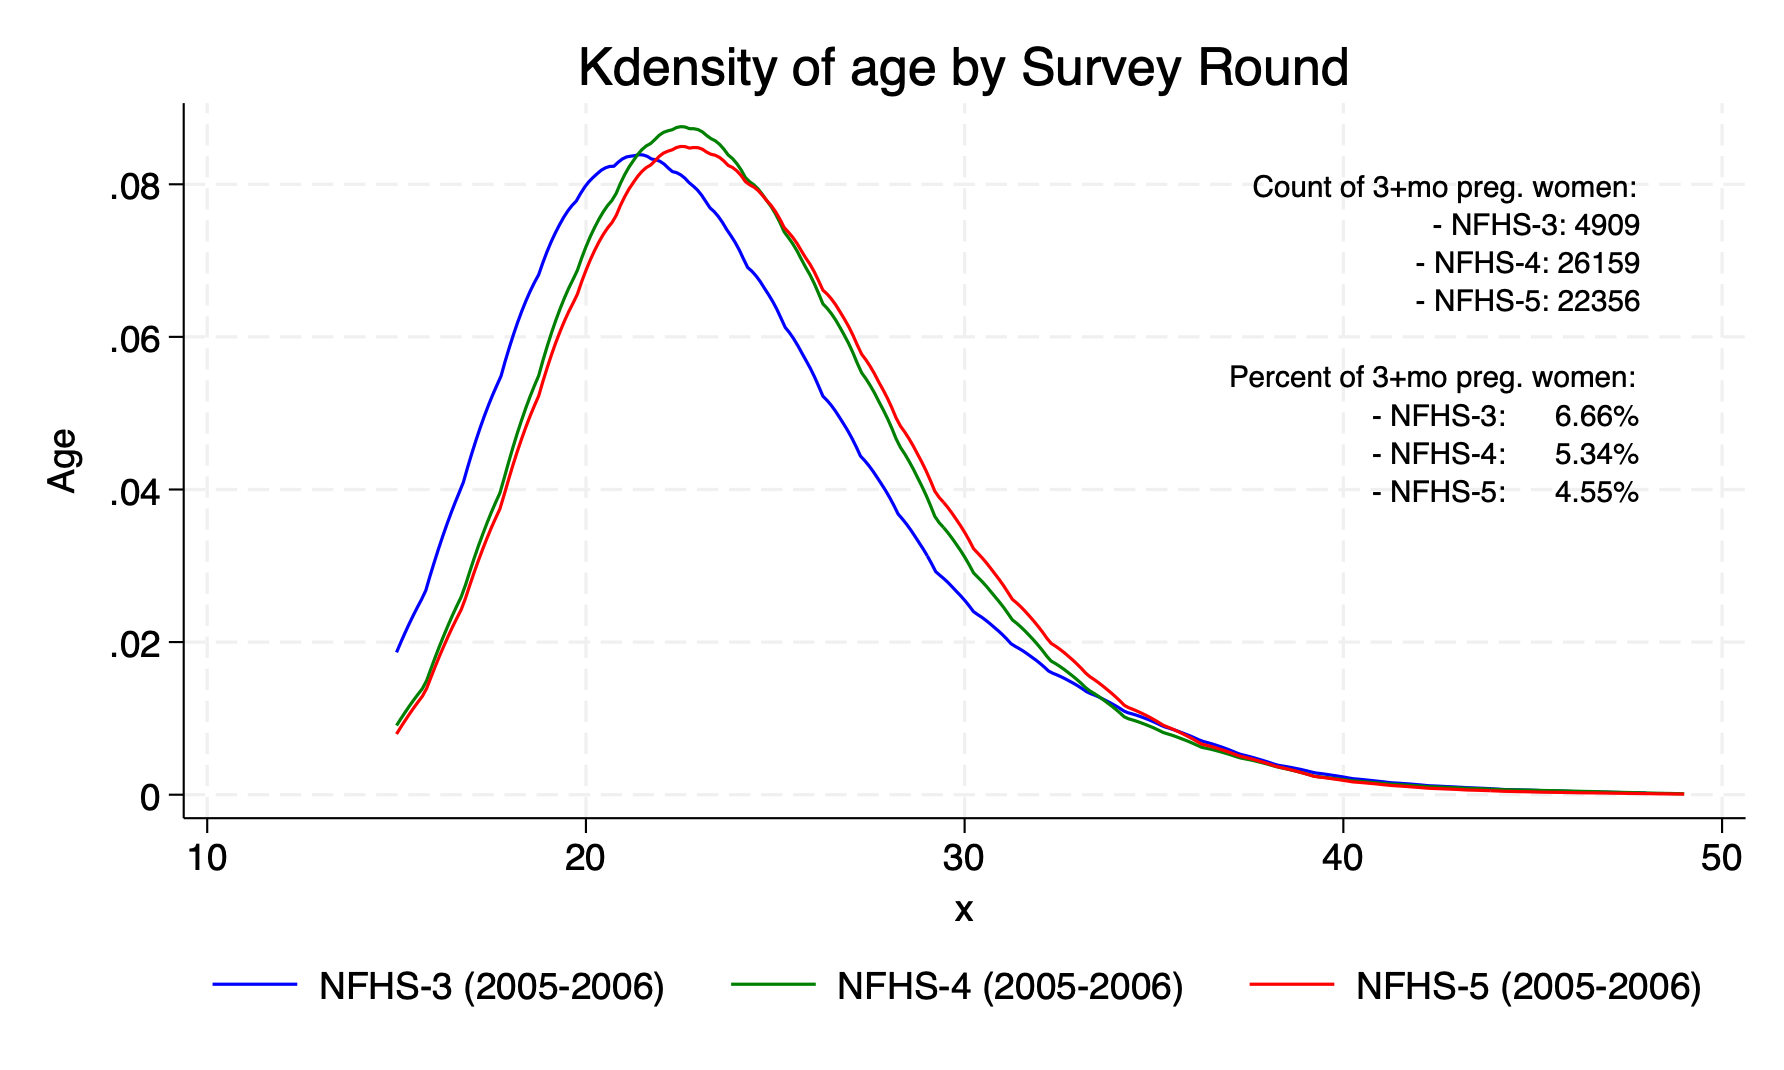
\includegraphics[width=\textwidth]{figures/kdensities ages.png}
    \caption{: Kernel density of the ages of currently pregnant women in NFHS 3, 4, \& 5}
\end{figure}


\begin{figure}[H]
    \centering
    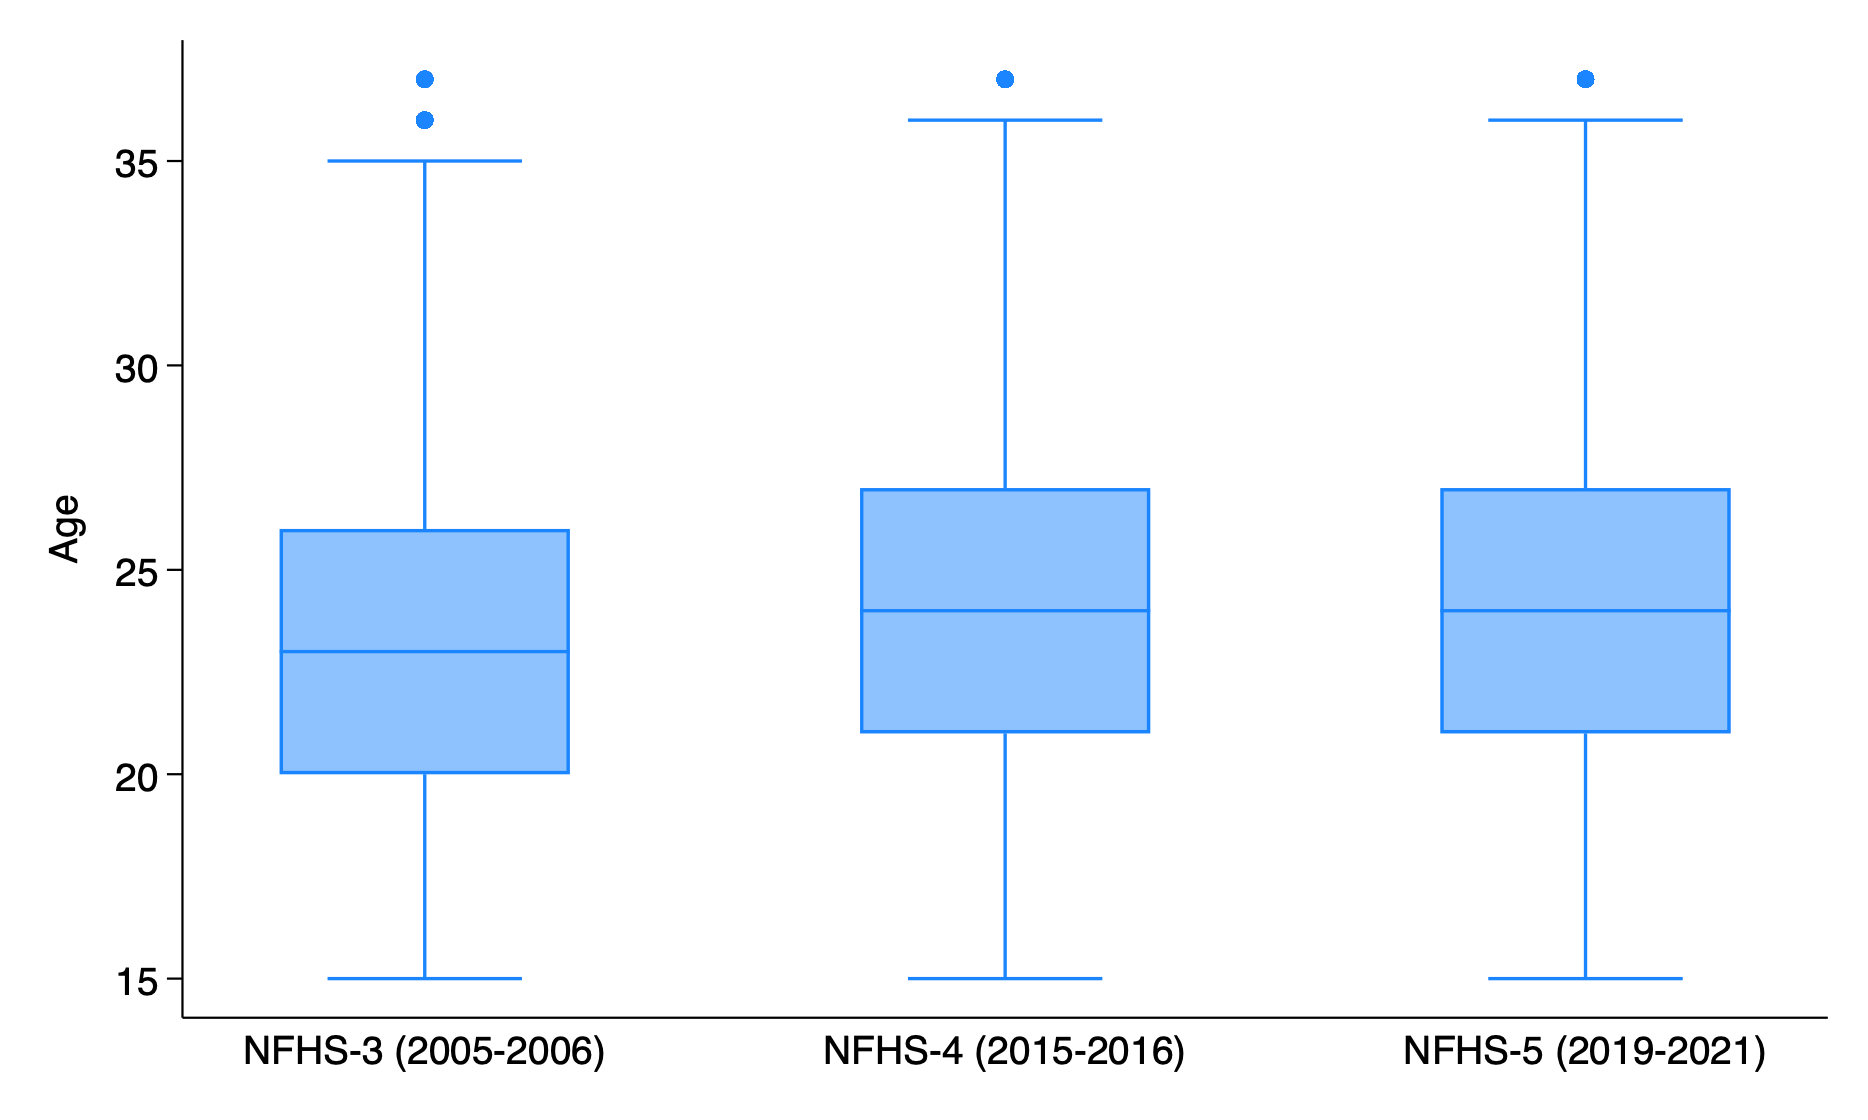
\includegraphics[width=\textwidth]{figures/boxplots ages.png}
    \caption{: Box plots of the age distributions of currently pregnant women NFHS 3, 4, \& 5}
\end{figure}

\begin{figure}[H]
    \centering
    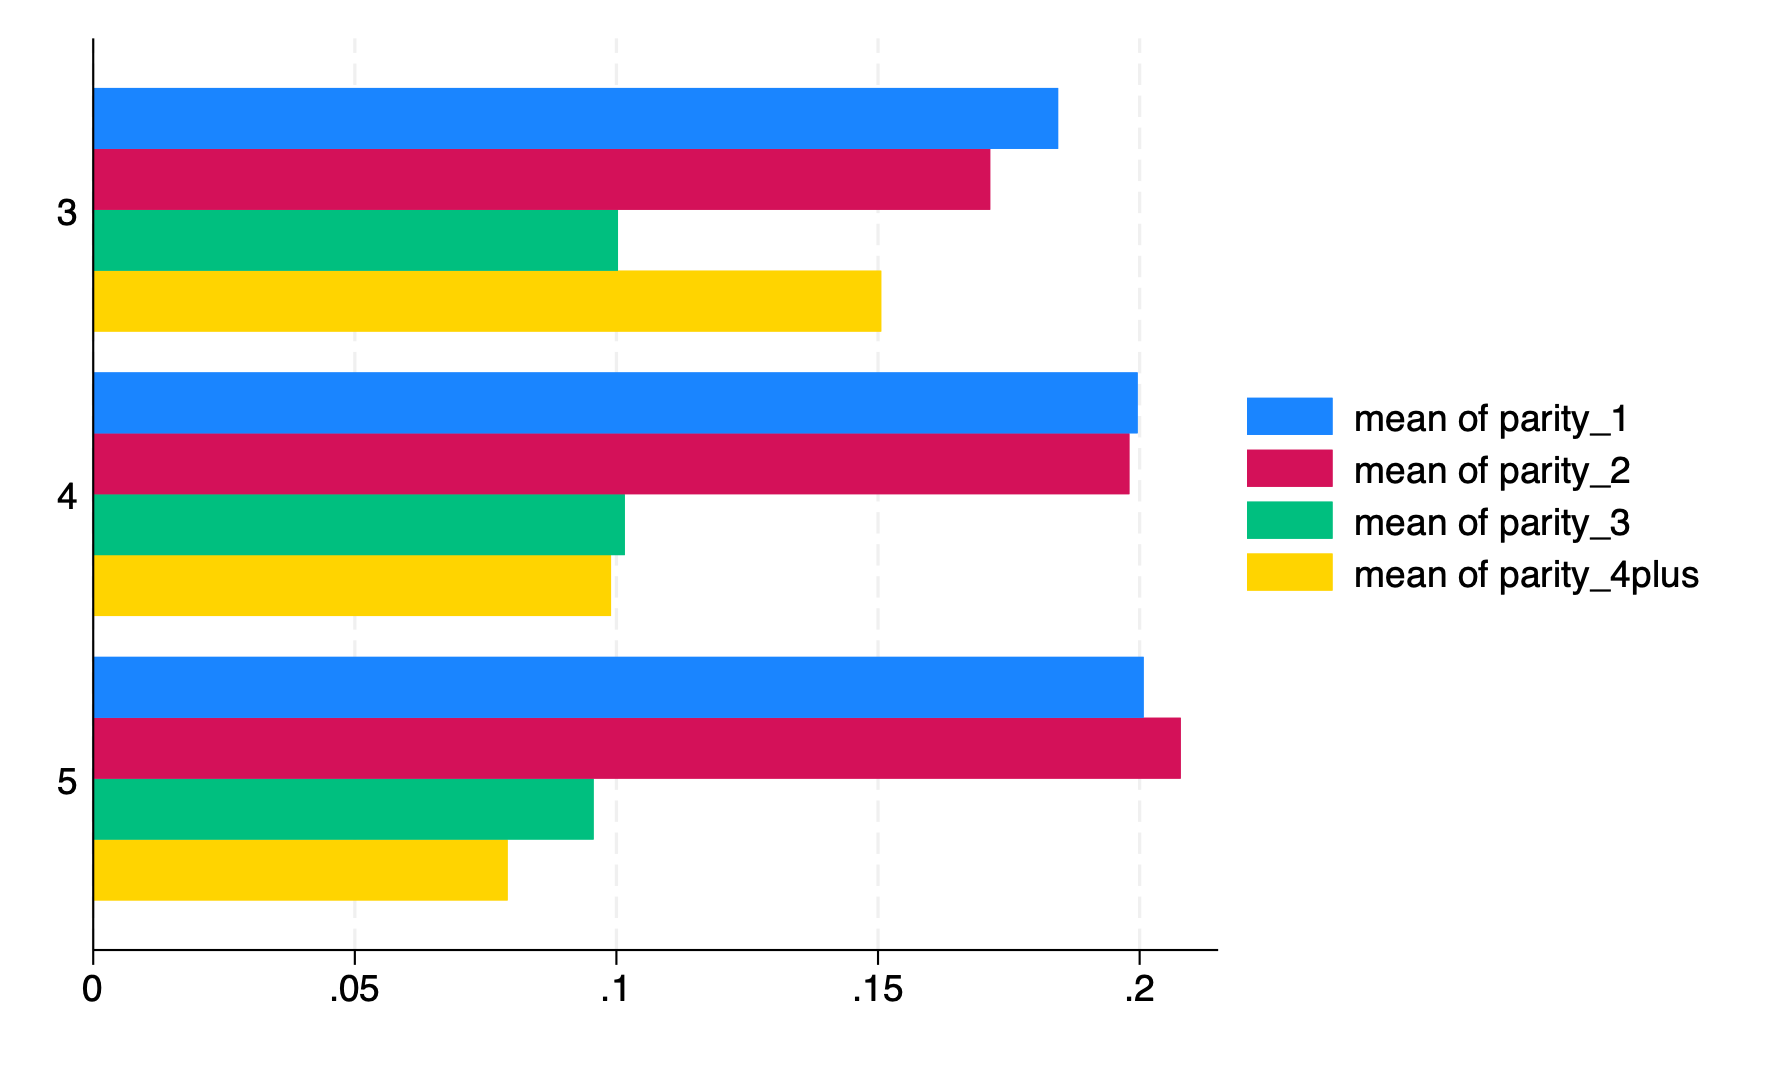
\includegraphics[width=\textwidth]{figures/bar graph number of children.png}
    \caption{: Bar graph of number of living children among currently pregnant women in the NFHS 3, 4, \& 5}
\end{figure}



TODO:
- total for all parities
\begin{table}[H]
    \centering
    \caption{: Proportion of pregnant women by gestational duration in the NFHS 3, 4, \& 5}
    \label{tab:sumstat}
    \adjustbox{width=\textwidth}{\begin{tabular}{l*{6}{c}}
\toprule
            &NFHS-3 (2005-2006)&            &NFHS-4 (2015-2016)&            &NFHS-5 (2019-2021)&            \\
            &\multicolumn{1}{c}{Mopreg}&\multicolumn{1}{c}{Moperiod}&\multicolumn{1}{c}{Mopreg}&\multicolumn{1}{c}{Moperiod}&\multicolumn{1}{c}{Mopreg}&\multicolumn{1}{c}{Moperiod}\\
\midrule
\midrule
1           &       1.807&       5.163&       4.602&       1.762&       4.987&       4.473\\
2           &       8.775&       8.199&       8.635&       8.696&       7.657&       8.285\\
3           &       13.44&       13.26&       12.38&       13.14&       12.51&       11.98\\
4           &       12.85&       12.83&       12.75&       12.74&       11.96&       12.37\\
5           &       12.73&       13.42&       12.21&       12.57&       12.60&       11.80\\
6           &       12.10&       12.19&       12.42&       11.86&       11.48&       11.82\\
7           &       11.84&       11.92&       12.00&       11.68&       11.20&       11.50\\
8           &       12.33&       12.02&       13.07&       12.14&       11.20&       12.26\\
9           &       11.28&       8.505&       9.477&       10.93&       7.918&       8.995\\
10          &       2.651&       2.060&       2.165&       2.638&       2.052&       2.144\\
11          &       0.196&       0.436&       0.277&       0.196&       0.436&       0.277\\
\bottomrule
\multicolumn{7}{l}{\footnotesize Mopreg refers to respondents self reported gestational duration. Moperiod refers months since last menstrual period.}\\
\end{tabular}
}
\end{table}


TODO:
- total for all parities
\begin{table}[H]
    \centering
    \caption{: Proportion of wanted pregnancies among pregnant women by parity in the NFHS 3, 4, \& 5}
    \label{tab:sumstat}
    \adjustbox{width=\textwidth}{{
\def\sym#1{\ifmmode^{#1}\else\(^{#1}\)\fi}
\begin{tabular}{l*{3}{c}}
\hline\hline
            &\multicolumn{1}{c}{NFHS-3}&\multicolumn{1}{c}{NFHS-4}&\multicolumn{1}{c}{NFHS-5}\\
\hline
\hline
Parity 1    &       85.14         &       94.99         &       94.85         \\
Parity 2    &       74.04         &       88.12         &       88.97         \\
Parity 3    &       71.06         &       80.72         &       81.92         \\
Parity 4+   &       55.21         &       69.60         &       74.63         \\
\hline\hline
\multicolumn{4}{l}{\footnotesize \textit{t} statistics in parentheses}\\
\multicolumn{4}{l}{\footnotesize \sym{*} \(p<0.05\), \sym{**} \(p<0.01\), \sym{***} \(p<0.001\)}\\
\end{tabular}
}
}
\end{table}


TODO: 
- make sure it's only non-pregnant women.
\begin{table}[H]
    \centering
    \caption{: Proportion of married women using modern contraception in the NFHS 3, 4, \& 5}
    \label{tab:sumstat}
    \adjustbox{width=\textwidth}{\begin{tabular}{l*{3}{c}}
\toprule
            &\multicolumn{1}{c}{NFHS-3 (2005–2006)}&\multicolumn{1}{c}{NFHS-4 (2015–2016)}&\multicolumn{1}{c}{NFHS-5 (2019–2021)}\\
\midrule
\midrule
No living boy child&       12.06&       15.33&       25.50\\
No children &       4.031&       6.664&       14.29\\
\bottomrule
\end{tabular}
}
\end{table}
Interpretation: women are more able to decide despite social pressure of having a boy/child

% \begin{figure}[H]
%     \centering
%     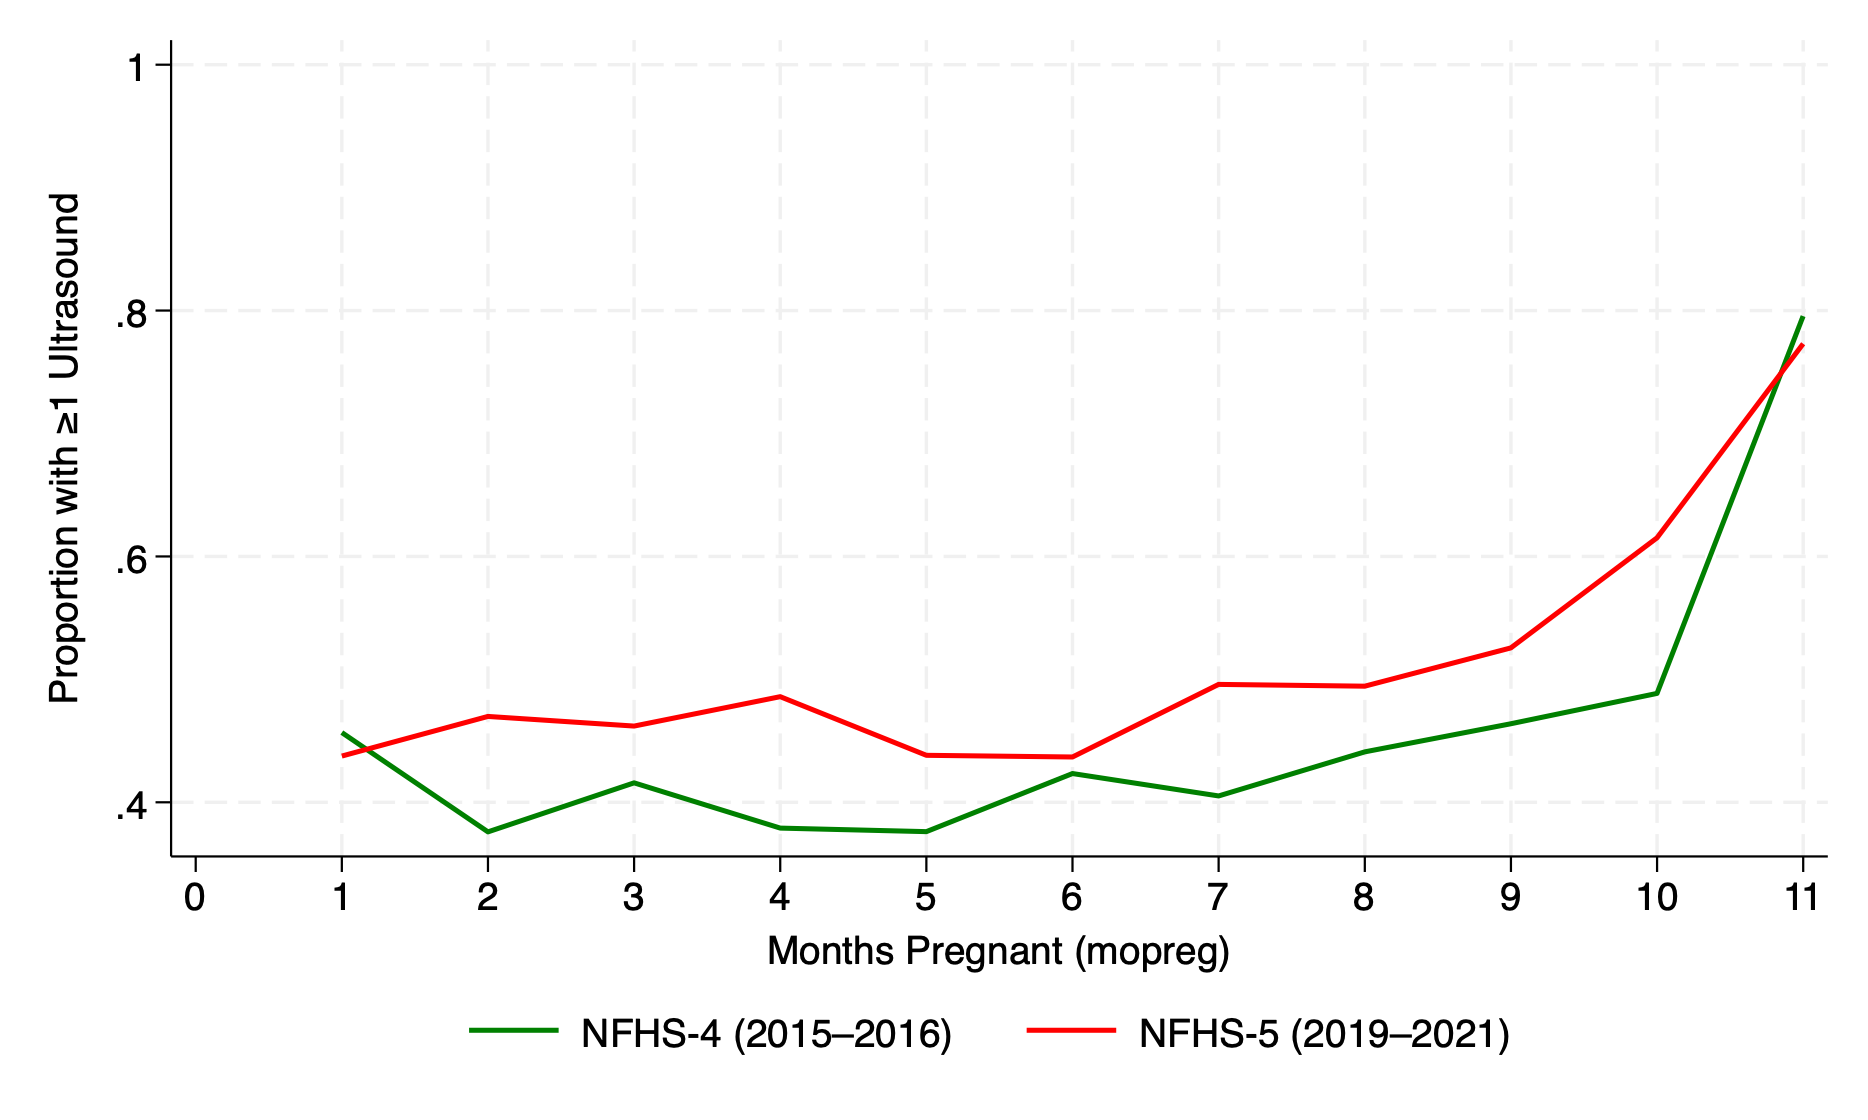
\includegraphics[width=\textwidth]{figures/ultrasound by pregnancy duration.png}
%     \caption{: Proportion of pregnant women who have had an ultrasound by gestational duration in NFHS 4, \& 5}
% \end{figure}

\begin{table}[H]
    \centering
    \caption{: Proportion of pregnant women who have had an ultrasound by gestational duration in NFHS 4, \& 5}
    \label{tab:sumstat}
\end{table}


\begin{figure}[H]
    \centering
    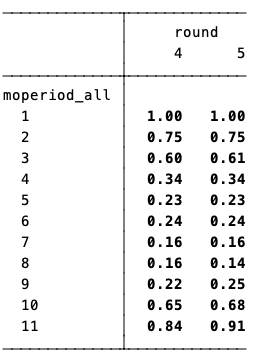
\includegraphics[width=\textwidth]{tables/says pregnant by gestational duration.png}
    \caption{: Proportion of women who report not being pregnant by months since last period in the NFHS 4, \& 5}
\end{figure}


\end{document}



fix lines on end-pregnancy BMI
remove titles on graphs from stata
label xaxis on kdensity age
maybe make stats on kdensity age separate table




- different living situations between pregnant, non-pregnant women (with reweighting), all non-pregnant women (without reweighting)
- create categories of household type accordingly
- model off: https://link.springer.com/article/10.1007/s13524-012-0173-1

- then get breakdown of proportion of pregnant



